\section{優美動作の評価}

\subsection{従来手法}
上田研ではこれまで多くのモデルが提唱されてきた.
その多くは稲津\cite{inazu2}の全曲率計算を起源としている.
先に挙げたB-spline近似で手先軌道を曲線近似し,図\ref{curves}のように
全曲率$\mu$が0.87〜1.31となる曲線を多く含むものを優美としている.
そこから面積や角度に派生するモデルも存在するが,根底は手先軌道である.
今回作成したネットワークが「優美」と判定したものは動画のどの箇所を根拠に
「優美」と判断したのか,動作を抽出して検証する際,どこに着目すべきと
示唆しているかなどを検証した.

\begin{figure}[b]
  \begin{center}
    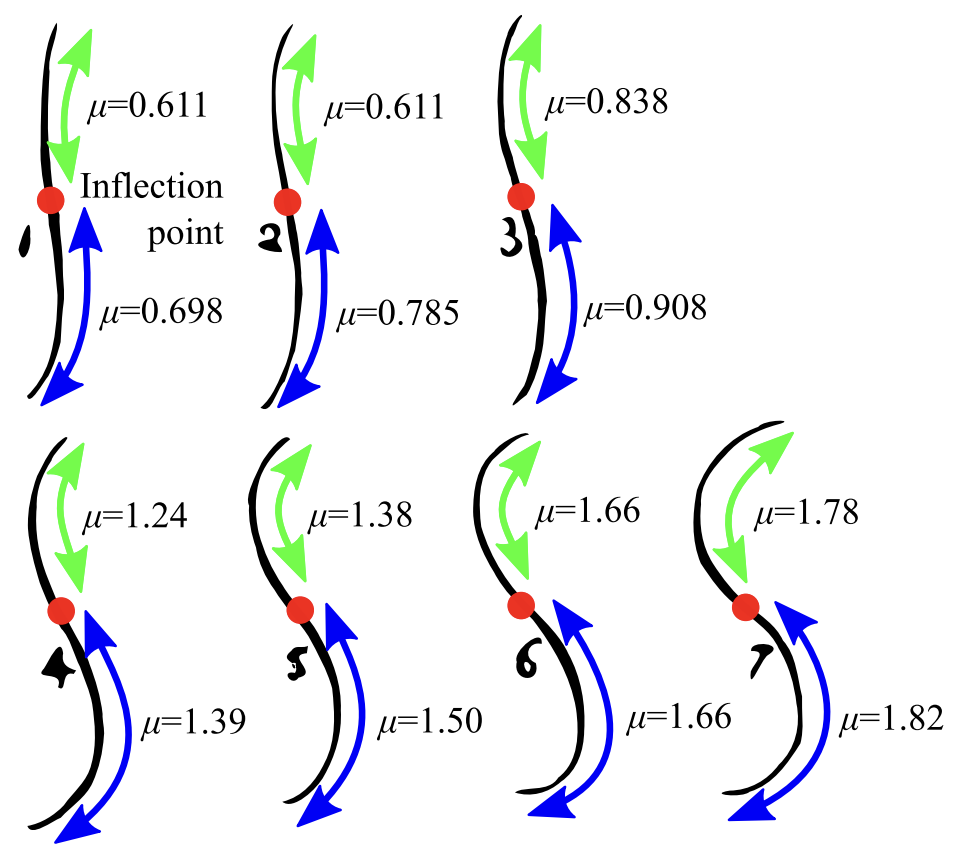
\includegraphics[width=100mm]{images/quote/curves.png}
  \end{center}
  \caption{Hogarth Curveの全曲率}
  \label{curves}
\end{figure}

\subsection{Grad Camを用いた評価}
作成したネットワークの判断根拠を可視化するために,Pytorch-GradCam\cite{pygradcam}を
使用した.作成したネットワークはPytorch\cite{pytorch}でできているので,GradCamも
同じくPytorchでできたものを使用した.Transformer

Pytorch-GradCamは入力データに対してどのように各層が影響するか順伝播で確認してから,
逆伝播で影響の強弱を1以下の数値で返す.今回のネットワークでは動画をフレーム毎に区切るので
1フレームずつ処理すると最大30回重複するデータが存在する.
よって出力された結果を順番に足し合わせ,特定のデータについて足し合わされた回数で各値を割ることで
データの均一化を図った.データは1以下にあるので255をかけることでデータの強弱を動画として可視化した.
また,数値は小さいが,データが離散しているので閾値0.4以下の値は0とした.

\begin{figure}[b]
  \begin{center}
    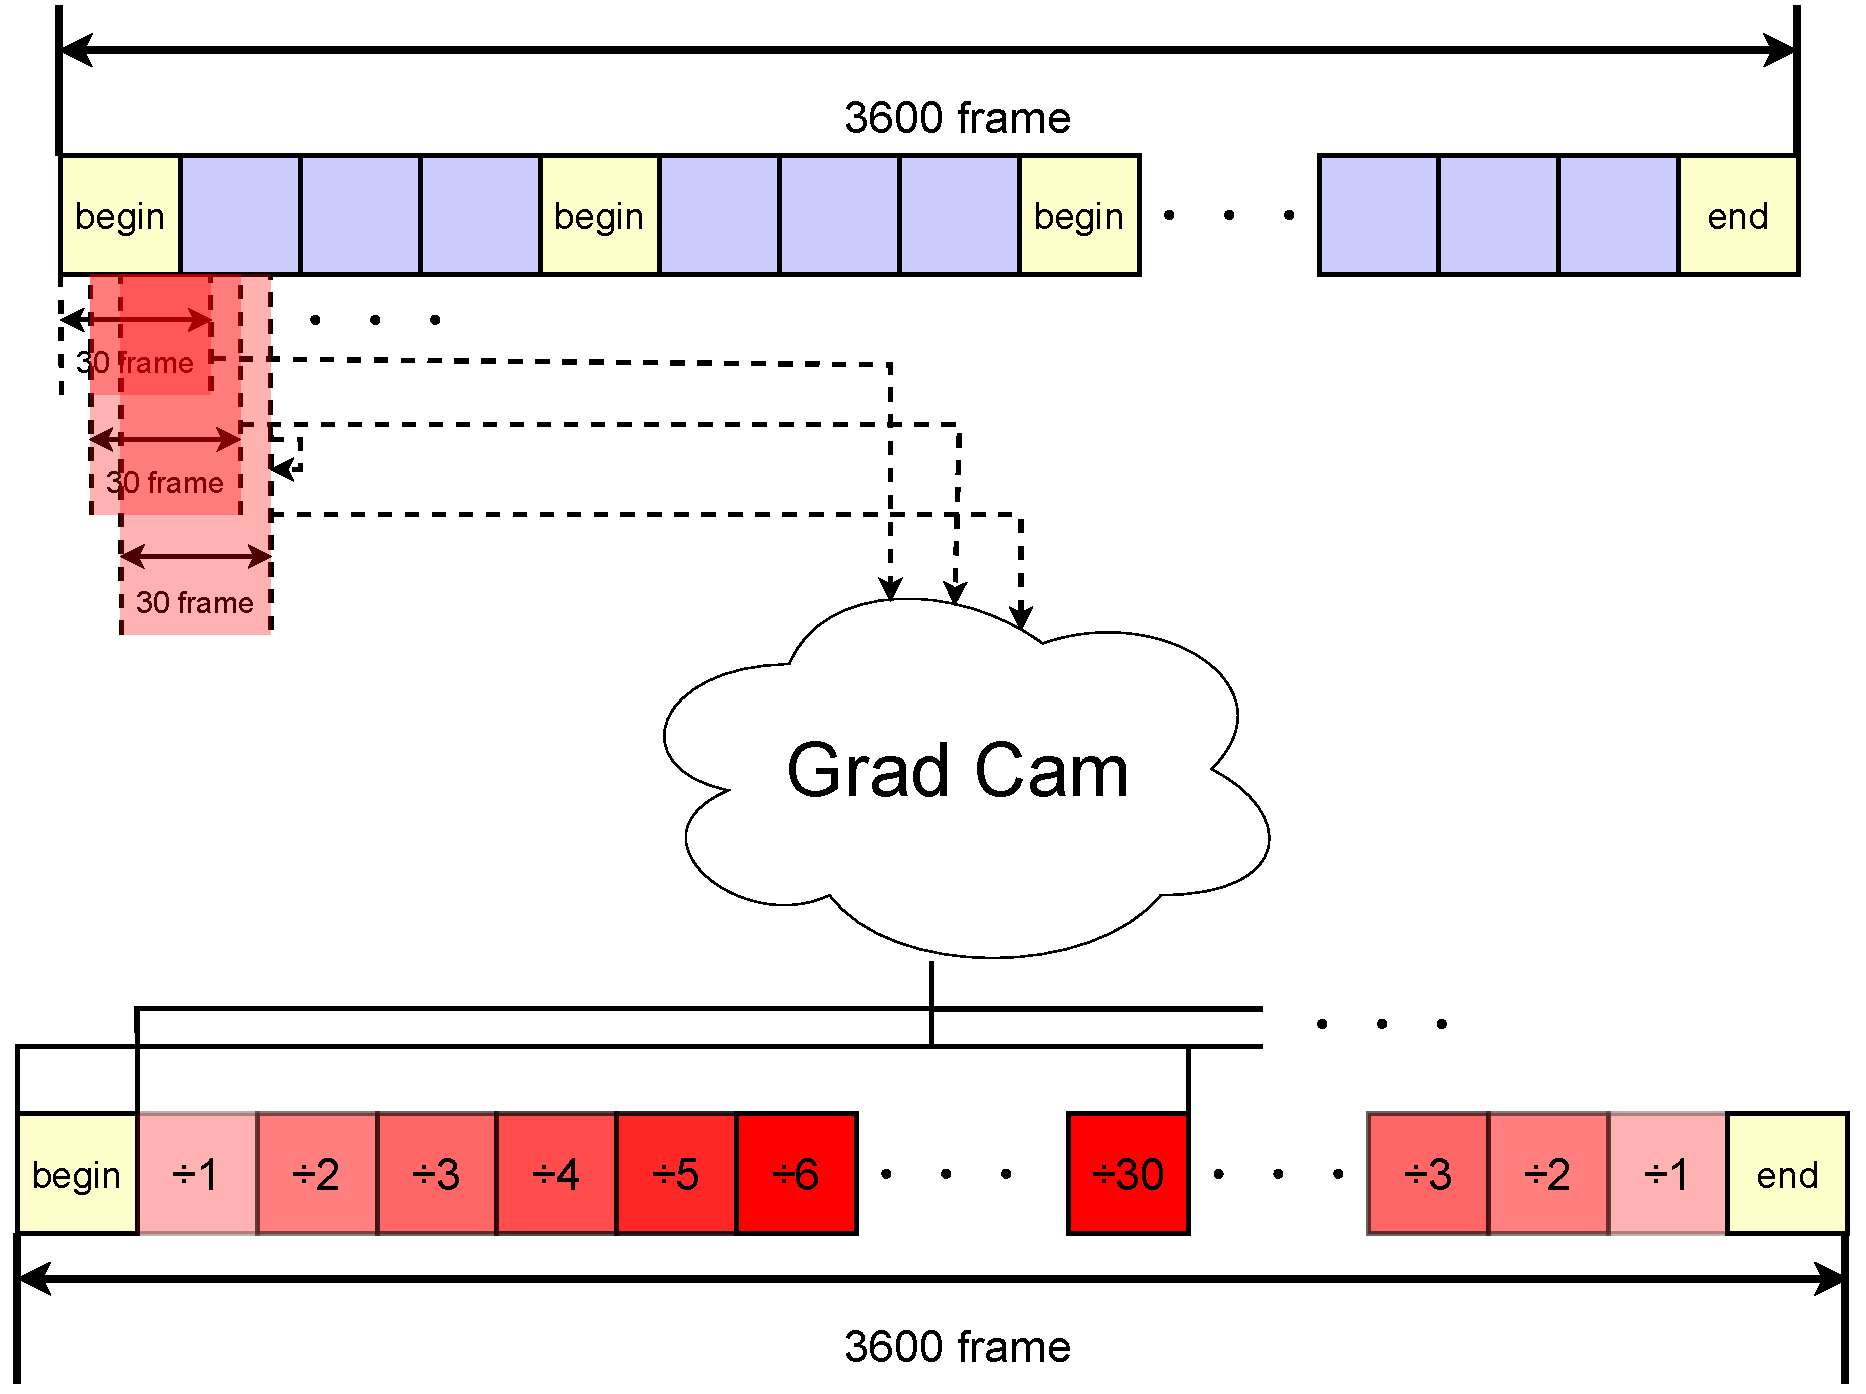
\includegraphics[width=120mm]{images/chart/gradcam.pdf}
  \end{center}
  \caption{Grad Camから出力される結果の整形方法}
  \label{gradcam}
\end{figure}
\clearpage

\subsection{確率分布を用いた評価}

\subsection{従来手法との比較}